\documentclass[conference]{IEEEtran}
\IEEEoverridecommandlockouts
% Este entorno no tiene las fuentes Times (psnfss) que IEEEtran fija por defecto;
% se revierte a Computer Modern (siempre disponible). Debe ir ANTES de todo paquete
% que dispare la carga de fuentes.
\renewcommand{\rmdefault}{cmr}
\renewcommand{\sfdefault}{cmss}
\renewcommand{\ttdefault}{cmtt}
\usepackage{cite}
\usepackage{amsmath,amssymb,amsfonts}
\usepackage{graphicx}
\usepackage{textcomp}
\usepackage{xcolor}
\usepackage[spanish,es-nodecimaldot]{babel}
\usepackage{booktabs}
\usepackage[hidelinks]{hyperref}
\graphicspath{{../../figures/}{../../figures/modeling/}}

\begin{document}

\title{Comparaci\'on Emp\'irica de Seis Clasificadores Supervisados para la
Predicci\'on Multiclase de Resultados de F\'utbol a Escala Multi-Liga (2000--2025)\\
{\footnotesize Curso: Miner\'ia de Datos (CC442) --- Ciclo Acad\'emico 2026-I ---
Prof. Dr. Marcos Antonio Alania Vicente}
}

\author{
\IEEEauthorblockN{Arb\'ues Enrique P\'erez Villegas}
\IEEEauthorblockA{\textit{Escuela de Ciencia de la Computaci\'on} \\
\textit{Universidad Nacional de Ingenier\'ia}\\
Lima, Per\'u \\
arbues.perez@uni.pe}
\and
\IEEEauthorblockN{Sergio Sebastian Pezo Jimenez}
\IEEEauthorblockA{\textit{Escuela de Ciencia de la Computaci\'on} \\
\textit{Universidad Nacional de Ingenier\'ia}\\
Lima, Per\'u \\
sergio.pezo@uni.pe}
\and
\IEEEauthorblockN{Luis Andre Trujillo Serva}
\IEEEauthorblockA{\textit{Escuela de Ciencia de la Computaci\'on} \\
\textit{Universidad Nacional de Ingenier\'ia}\\
Lima, Per\'u \\
luis.trujillo@uni.pe}
}

\maketitle

\begin{abstract}
La predicci\'on del resultado de un partido de f\'utbol (victoria local, empate o
victoria visitante) es un problema de clasificaci\'on multiclase notoriamente dif\'icil
por el peso del azar y por la clase minoritaria del empate. La literatura previa alcanza
gran escala usando m\'etricas probabil\'isticas y pocos algoritmos, o compara
clasificadores con m\'etricas est\'andar sobre conjuntos peque\~nos; ninguna ofrece una
comparaci\'on amplia de clasificadores modernos con m\'etricas por clase y prueba de
significancia a gran escala. Este trabajo eval\'ua de forma controlada nueve familias de
modelos (desde una l\'inea base ingenua hasta ensambles apilados) sobre 230\,554 partidos
de m\'ultiples ligas (2000--2025), empleando exclusivamente informaci\'on previa al
partido y sin cuotas de mercado. Se adopta un protocolo de validaci\'on estrictamente
temporal y se optimiza la m\'etrica F1 macro por el desbalance de clases. El ensamble por
apilamiento propuesto alcanza un F1 macro de 0,419 en el conjunto de prueba y supera a las
l\'ineas base con significancia estad\'istica (prueba de Wilcoxon, $p<0{,}001$). Se
demuestra emp\'iricamente que la frontera del empate es no lineal, que el reponderado por
clase supera al sobremuestreo sint\'etico, y que la diferencia de \emph{rating} Elo es la
variable dominante seg\'un an\'alisis SHAP. Los resultados confirman un techo de
rendimiento honesto coherente con el estado del arte y aportan una comparaci\'on
reproducible que la literatura no ten\'ia.
\end{abstract}

\begin{IEEEkeywords}
aprendizaje autom\'atico, clasificaci\'on multiclase, desbalance de clases,
gradient boosting, predicci\'on deportiva, validaci\'on temporal
\end{IEEEkeywords}

\section{Introducci\'on}
La industria del f\'utbol mueve cifras econ\'omicas de gran magnitud y ha convertido la
anal\'itica deportiva en una disciplina de inter\'es cient\'ifico e industrial. Predecir
el resultado de un encuentro tiene aplicaciones en la gesti\'on deportiva, los mercados de
apuestas y la generaci\'on de contenido; sin embargo, sigue siendo un problema abierto por
la alta componente estoc\'astica del juego y por la dificultad estructural de la clase
``empate''.

Formalmente, se aborda un problema de clasificaci\'on supervisada multiclase. Dado un
vector de caracter\'isticas $\mathbf{x}\in\mathbb{R}^{d}$ construido con informaci\'on
disponible \emph{antes} del inicio del partido, se busca una hip\'otesis
$g:\mathbb{R}^{d}\rightarrow\{H,D,A\}$ que asigne la etiqueta correcta, donde $H$ denota
victoria local, $D$ empate y $A$ victoria visitante. El objetivo es aprender $g$
minimizando el error de generalizaci\'on sobre partidos futuros, sin incurrir en fuga de
informaci\'on temporal.

La motivaci\'on t\'ecnica de este estudio nace de una brecha concreta en la literatura
(Secci\'on~\ref{sec:related}): los trabajos que operan a gran escala emplean m\'etricas
probabil\'isticas como el \emph{Ranked Probability Score} y un repertorio reducido de
algoritmos, mientras que los que comparan clasificadores con m\'etricas est\'andar utilizan
conjuntos de datos peque\~nos. Este trabajo cierra esa brecha con una evaluaci\'on amplia,
por clase y con contraste de significancia, sobre un conjunto de gran escala.

Las contribuciones concretas son las siguientes:
\begin{enumerate}
\item Una comparaci\'on emp\'irica controlada de nueve familias de clasificadores
      ---incluyendo los tres motores modernos de \emph{gradient boosting}
      (XGBoost, LightGBM y CatBoost) y ensambles de tipo \emph{voting} y
      \emph{stacking}--- sobre 230\,554 partidos multi-liga, con reproducibilidad
      determinista y c\'omputo en GPU.
\item Un protocolo de evaluaci\'on honesto para datos desbalanceados y con deriva
      temporal: partici\'on por fecha, validaci\'on con \texttt{TimeSeriesSplit},
      optimizaci\'on de F1 macro y reporte por clase con prueba de Wilcoxon.
\item Evidencia experimental sobre tres cuestiones metodol\'ogicas: la naturaleza no
      lineal de la frontera del empate, la superioridad del reponderado por clase frente
      al sobremuestreo sint\'etico SMOTE, y la dominancia del \emph{rating} Elo v\'ia
      an\'alisis SHAP.
\end{enumerate}

El resto de este art\'iculo se organiza de la siguiente manera: la Secci\'on~\ref{sec:related}
revisa el estado del arte; la Secci\'on~\ref{sec:dataset} describe el conjunto de datos y
el an\'alisis exploratorio; la Secci\'on~\ref{sec:preproc} detalla el preprocesamiento; la
Secci\'on~\ref{sec:method} formaliza la metodolog\'ia y los modelos; la
Secci\'on~\ref{sec:software} documenta la implementaci\'on; la Secci\'on~\ref{sec:results}
presenta los resultados y el an\'alisis estad\'istico; la Secci\'on~\ref{sec:discussion}
discute los hallazgos y las amenazas a la validez; y la Secci\'on~\ref{sec:conclusions}
concluye.

\section{Trabajos Relacionados}\label{sec:related}
La predicci\'on de resultados de f\'utbol mediante aprendizaje autom\'atico cuenta con una
literatura consolidada. Rodrigues y Pinto~\cite{rodrigues2022} comparan ocho clasificadores
sobre la \emph{Premier League} y reportan un mejor resultado con \emph{Random Forest}
(exactitud del 65\%), con la salvedad de que el empate obtiene una sensibilidad muy baja
($\approx 30\%$). Choi \emph{et al.}~\cite{choi2023} estudian el efecto del muestreo y
concluyen que el \emph{balanced sampling} permite predecir empates que el muestreo
estratificado ignora. Ren y Susnjak~\cite{ren2022} comparan modelos incluyendo CatBoost,
\emph{voting} y \emph{stacking}, y obtienen un 51,9\% de exactitud global, con hasta un
70\% en partidos catalogados como ``f\'aciles''. Yeung \emph{et al.}~\cite{yeung2023}
reportan, con XGBoost sobre \emph{features} interpretables, un F1 de 0,47 y una exactitud
de 0,57, superando a las cuotas del mercado.

En el extremo de gran escala, Berrar \emph{et al.}~\cite{berrar2019,berrar2024} trabajan
con 216\,000 y m\'as de 300\,000 partidos de decenas de ligas usando datos ``simples''
(fecha, equipos, liga y marcador), pero eval\'uan con el \emph{Ranked Probability Score} y
un repertorio reducido de algoritmos (principalmente $k$-NN y \emph{boosting}); en su
edici\'on de 2024, ni el mejor modelo logr\'o batir al operador de apuestas. St\"ubinger
\emph{et al.}~\cite{stubinger2020} alcanzan una exactitud del 81,8\%, pero mediante una
\emph{regresi\'on} de la diferencia de goles con empates excluidos, por lo que su cifra no
es comparable con una clasificaci\'on de tres v\'ias. Atta Mills \emph{et al.}~\cite{attamills2024}
obtienen 0,83 de exactitud con un ensamble \emph{voting}, aunque incorporando
\emph{features} de medio tiempo (\emph{in-game}) que no est\'an disponibles antes del
partido. En el plano metodol\'ogico, Bunker y Thabtah~\cite{bunker2019} advierten
expl\'icitamente contra la validaci\'on cruzada aleatoria en datos con orden temporal y
proponen esquemas por rondas, recomendaci\'on reforzada por Bunker \emph{et al.}~\cite{bunker2024}.

Es preciso advertir que estas cifras \emph{no} son directamente comparables entre s\'i,
pues los trabajos emplean formulaciones y m\'etricas heterog\'eneas ---clasificaci\'on de
tres v\'ias, regresi\'on de la diferencia de goles o puntajes probabil\'isticos--- y
subconjuntos de dificultad dispar. Contrastar la exactitud de una regresi\'on con empates
excluidos frente a una clasificaci\'on multiclase equivaldr\'ia a comparar magnitudes
distintas. Por ello, el presente estudio fija de antemano un protocolo \'unico
(clasificaci\'on H/D/A, m\'etricas por clase y validaci\'on temporal) y reporta el techo
honesto que le corresponde.

La Tabla~\ref{tab:gap} sintetiza esta comparaci\'on. Del contraste emergen tres consensos:
(i)~el empate es la clase m\'as dif\'icil, con sensibilidad t\'ipicamente inferior al
35\%; (ii)~el techo realista de exactitud previa al partido en tres clases se sit\'ua en
torno al 52--57\%; y (iii)~los m\'etodos basados en \'arboles (\emph{Random Forest} y
\emph{gradient boosting}) son ganadores recurrentes. La brecha que este trabajo aborda es
clara: ning\'un estudio compara simult\'aneamente seis clasificadores modernos ---incluidos
LightGBM y CatBoost--- con m\'etricas por clase y prueba de significancia sobre un conjunto
de escala superior a 200\,000 partidos multi-liga.

\begin{table}[t]
\caption{S\'intesis del estado del arte y brecha identificada}
\label{tab:gap}
\centering
\footnotesize
\begin{tabular}{@{}p{1.5cm}p{1.1cm}p{1.5cm}p{2.5cm}@{}}
\toprule
\textbf{Trabajo} & \textbf{Escala} & \textbf{M\'etrica} & \textbf{Mejor modelo / brecha} \\
\midrule
Rodrigues \cite{rodrigues2022} & 1\,900 & Acc, F1 & RF, Acc 0,65 \\
Choi \cite{choi2023} & 3\,297 & Acc, F1, AUC & LogReg mult., Acc 0,54 \\
Ren \cite{ren2022} & 1\,140 & Acc, P/R/F1 & CatBoost, Acc 0,52 \\
Yeung \cite{yeung2023} & 1\,700 & F1, AUC, Acc & XGBoost, F1 0,47 \\
Berrar \cite{berrar2019} & 216\,743 & RPS & $k$-NN, RPS 0,205 \\
Atta Mills \cite{attamills2024} & 1\,411 & Acc, F1 & Voting, Acc 0,83$^{\dagger}$ \\
\midrule
\textbf{Este trabajo} & \textbf{230\,554} & \textbf{F1/$\kappa$/AUC} & \textbf{Stacking + Wilcoxon} \\
\bottomrule
\end{tabular}

\vspace{3pt}
{\footnotesize\raggedright $^{\dagger}$Emplea \emph{features} de medio tiempo, no
comparables con predicci\'on estrictamente previa al partido.\par}
\end{table}

\section{Descripci\'on del Conjunto de Datos y An\'alisis Exploratorio}\label{sec:dataset}
Se emplea el conjunto p\'ublico \emph{Club Football Match Data (2000--2025)}, que re\'une
230\,557 partidos de m\'ultiples ligas internacionales con 48 columnas originales, entre
ellas \emph{ratings} Elo, forma reciente, estad\'isticas del partido y cuotas de mercado.
La variable objetivo es \texttt{FTResult}$\in\{H,D,A\}$. Tras eliminar tres registros sin
etiqueta, el conjunto operativo asciende a 230\,554 instancias.

El an\'alisis exploratorio revela cuatro propiedades que condicionan todo el modelado.
Primero, existe un \textbf{desbalance moderado} (Fig.~\ref{fig:balance}): la victoria local
representa el 44,6\%, la visitante el 28,9\% y el empate el 26,5\%, con una raz\'on de
desbalance de 1,68. Este r\'egimen desaconseja optimizar la exactitud, pues un clasificador
que siempre prediga ``local'' ya alcanzar\'ia $\approx 44\%$.

\begin{figure}[t]
\centering
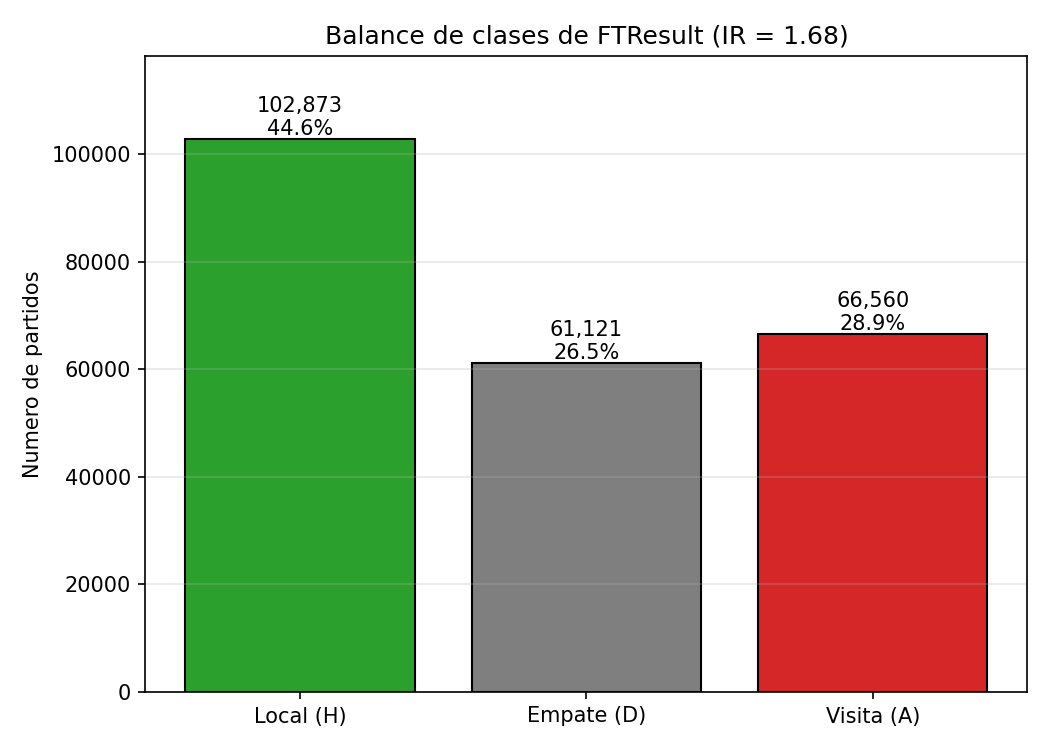
\includegraphics[width=0.86\linewidth]{class_balance.png}
\caption{Distribuci\'on de la variable objetivo. La victoria local domina y el empate es la
clase minoritaria, lo que motiva optimizar F1 macro en lugar de exactitud.}
\label{fig:balance}
\end{figure}

Segundo, la se\~nal principal es la \textbf{diferencia de Elo}: al ordenar los partidos por
esta variable, la tasa de victoria local, empate y visitante se separa de forma mon\'otona,
pero el empate queda siempre en la zona central sin dominar ninguna regi\'on
(Fig.~\ref{fig:elo}). Esto anticipa una \textbf{frontera de decisi\'on no lineal} alrededor
del cero, favorable a \'arboles y \emph{kernels}. Tercero, se detecta
\textbf{multicolinealidad exacta}: las variables de diferencia son combinaciones lineales
de sus componentes, lo que se traduce en factores de inflaci\'on de varianza infinitos y en
autovalores nulos del an\'alisis de componentes principales. Cuarto, el \emph{rating} Elo
presenta ausencias \textbf{estructurales por liga} (las competiciones no europeas carecen
de \'el) y el conjunto exhibe \textbf{deriva temporal}, con una ca\'ida de la ventaja local
durante la pandemia.

\begin{figure}[t]
\centering
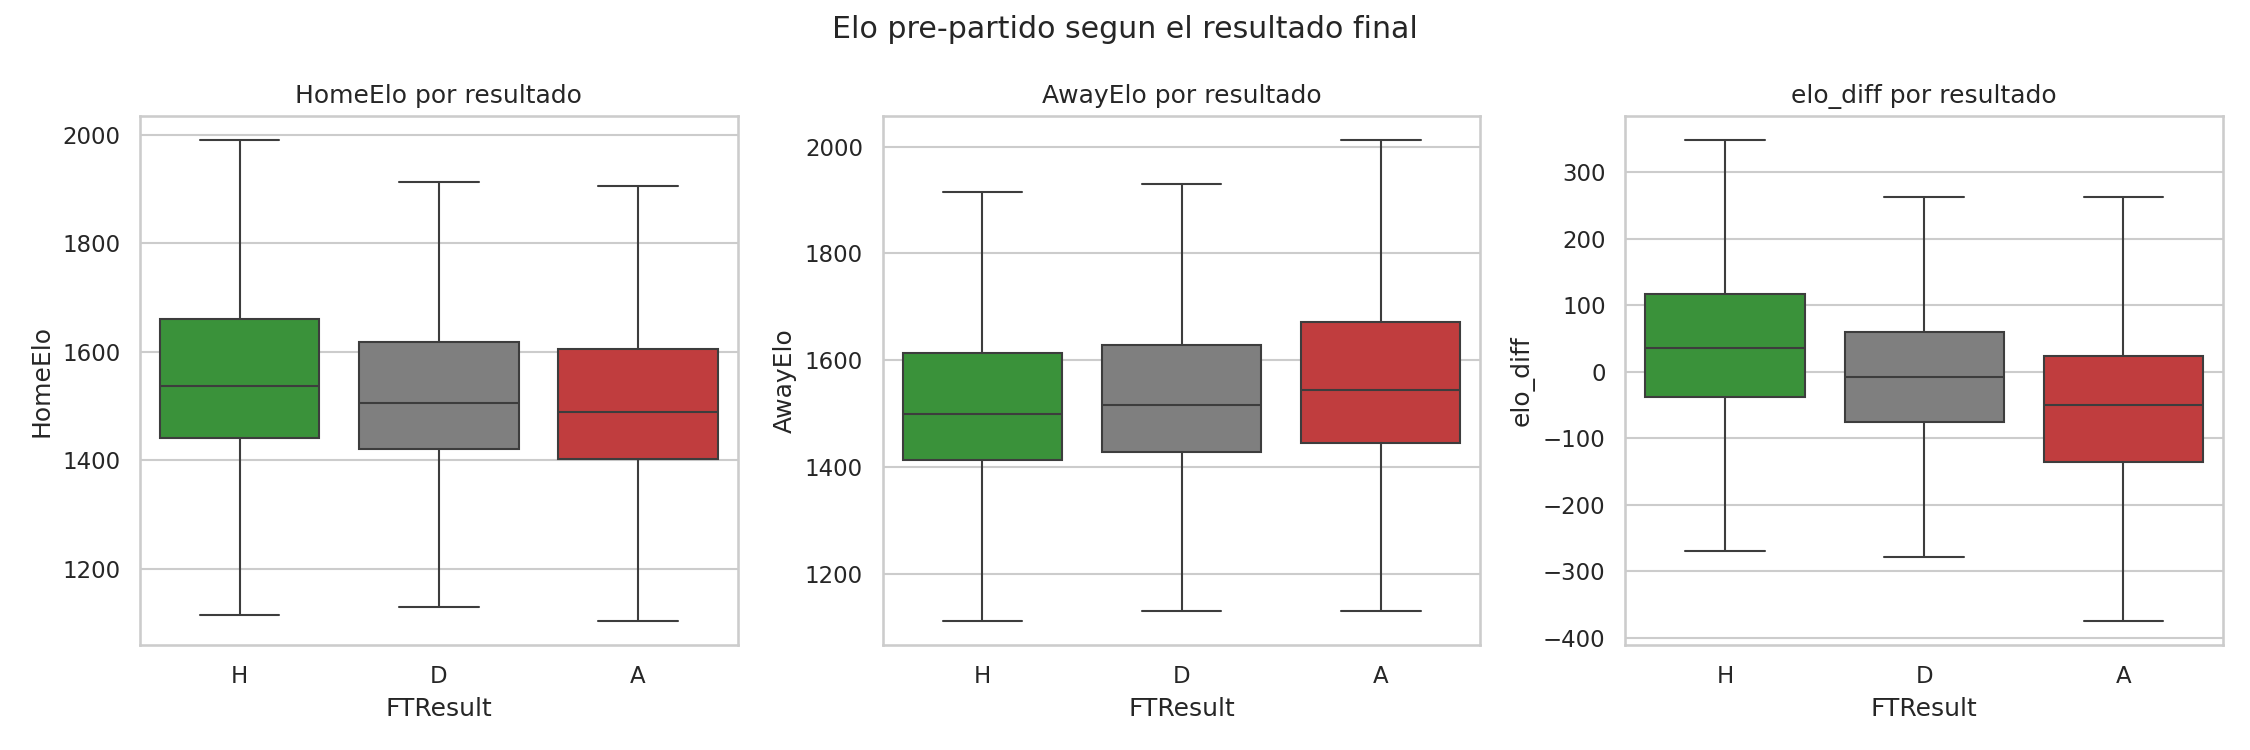
\includegraphics[width=0.86\linewidth]{elo_by_result.png}
\caption{Distribuci\'on del Elo por resultado. La diferencia de calidad separa los tres
resultados, pero el empate carece de una regi\'on propia, lo que fija un techo estructural
a su sensibilidad.}
\label{fig:elo}
\end{figure}

La Tabla~\ref{tab:dict} resume el diccionario de las 62 variables resultantes de la
ingenier\'ia de \emph{features}, agrupadas por naturaleza. Todas se calculan con
informaci\'on estrictamente anterior a cada partido.

\begin{table}[t]
\caption{Diccionario de variables de la matriz final (62 caracter\'isticas)}
\label{tab:dict}
\centering
\footnotesize
\begin{tabular}{@{}p{2.1cm}p{1.1cm}p{3.9cm}@{}}
\toprule
\textbf{Grupo (n)} & \textbf{Tipo} & \textbf{Descripci\'on} \\
\midrule
Elo (2) & continua & \emph{rating} Elo de local y visitante \\
Forma (4) & continua & puntos en los \'ultimos 3 y 5 partidos \\
Goles \emph{rolling} (4) & continua & promedio de goles a favor y en contra (5) \\
Diferencias (5) & continua & Elo, forma 3/5 y goles a favor/contra \\
Contexto (7) & continua & descanso, rachas e historial directo \\
Banderas (2) & binaria & liga top y Elo ausente \\
Liga (38) & \emph{one-hot} & divisi\'on del partido \\
\bottomrule
\end{tabular}
\end{table}

La estructura de correlaci\'on lineal (Fig.~\ref{fig:corr}) hace visible la
multicolinealidad: las variables de diferencia forman bloques de correlaci\'on perfecta con
sus componentes, lo que anticipa la necesidad de regularizar los modelos lineales.

\begin{figure}[t]
\centering
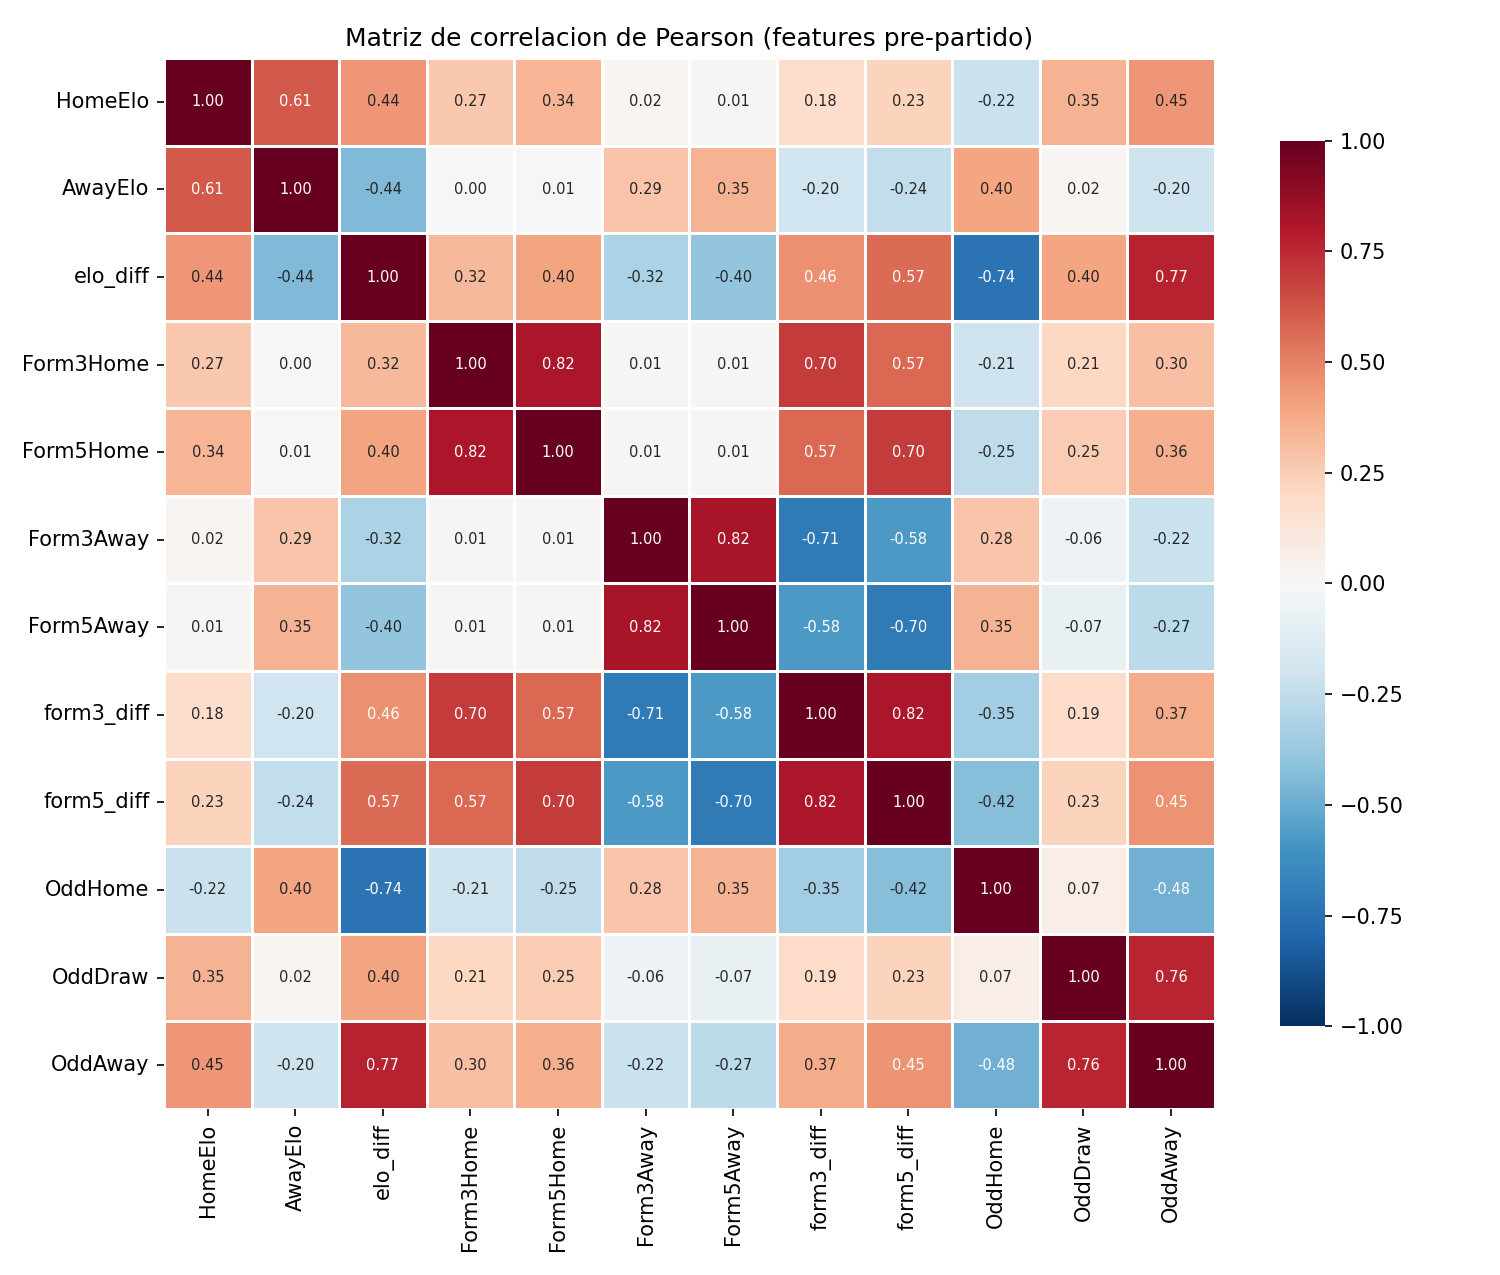
\includegraphics[width=0.94\linewidth]{correlation_matrix.png}
\caption{Matriz de correlaci\'on lineal de las variables num\'ericas. Los bloques de
correlaci\'on perfecta corresponden a las variables de diferencia y sus componentes,
origen de la multicolinealidad exacta.}
\label{fig:corr}
\end{figure}

\section{Preprocesamiento y Justificaci\'on Matem\'atica}\label{sec:preproc}
El preprocesamiento se dise\~n\'o para respetar la higiene anti-fuga exigida por la
naturaleza temporal del problema. Se descartaron las columnas posteriores al partido
(estad\'isticas de juego, marcador y variables de medio tiempo), que constituyen fuga
directa, y ---por decisi\'on de dise\~no--- las cuotas de mercado, con el fin de evaluar el
poder predictivo ``honesto'' del sistema sin la muleta del operador de apuestas.

El \emph{rating} Elo se reconstruy\'o mediante una uni\'on temporal (\emph{merge-asof}) con
la restricci\'on $\text{fecha}\le\text{fecha del partido}$ para evitar fuga, y las ausencias
estructurales se se\~nalizaron con una bandera expl\'icita. A partir de las variables
seguras se construy\'o un conjunto de \emph{features} de ingenier\'ia ---diferencia de Elo,
forma reciente, promedios m\'oviles de goles a favor y en contra, historial directo, d\'ias
de descanso, rachas y pertenencia a liga top--- calculados \'unicamente con partidos
anteriores a cada fila.

La partici\'on es \textbf{estrictamente temporal}: entrenamiento hasta 2021 (191\,099
instancias), validaci\'on 2022--2023 (24\,669) y prueba 2024--2025 (14\,786), con frontera
verificada. La justificaci\'on te\'orica es la desigualdad de generalizaci\'on: la cota de
Vapnik--Chervonenkis exige fijar la hip\'otesis \emph{antes} de tocar el conjunto de
evaluaci\'on, y una validaci\'on cruzada aleatoria sobre datos temporales introducir\'ia
partidos del futuro en el entrenamiento, sesgando la estimaci\'on del error.

La estandarizaci\'on de las variables continuas se calcul\'o \textbf{solo sobre el
entrenamiento} y se aplic\'o de forma ciega al resto:
\begin{equation}
x'_{ij} = \frac{x_{ij}-\mu_j}{\sigma_j},
\end{equation}
donde $\mu_j$ y $\sigma_j$ son la media y la desviaci\'on est\'andar de la caracter\'istica
$j$ estimadas en el entrenamiento. Las variables de liga se codificaron con
\emph{one-hot}, resultando una matriz final de \textbf{62 caracter\'isticas}. Como control
de la multicolinealidad, se computa un an\'alisis de componentes principales sobre las
variables continuas: la varianza acumulada alcanza el 95\% con 13 componentes
(Fig.~\ref{fig:pca}), y aparecen cinco autovalores nulos que confirman las cinco
dependencias lineales exactas detectadas en el an\'alisis exploratorio.

\begin{figure}[t]
\centering
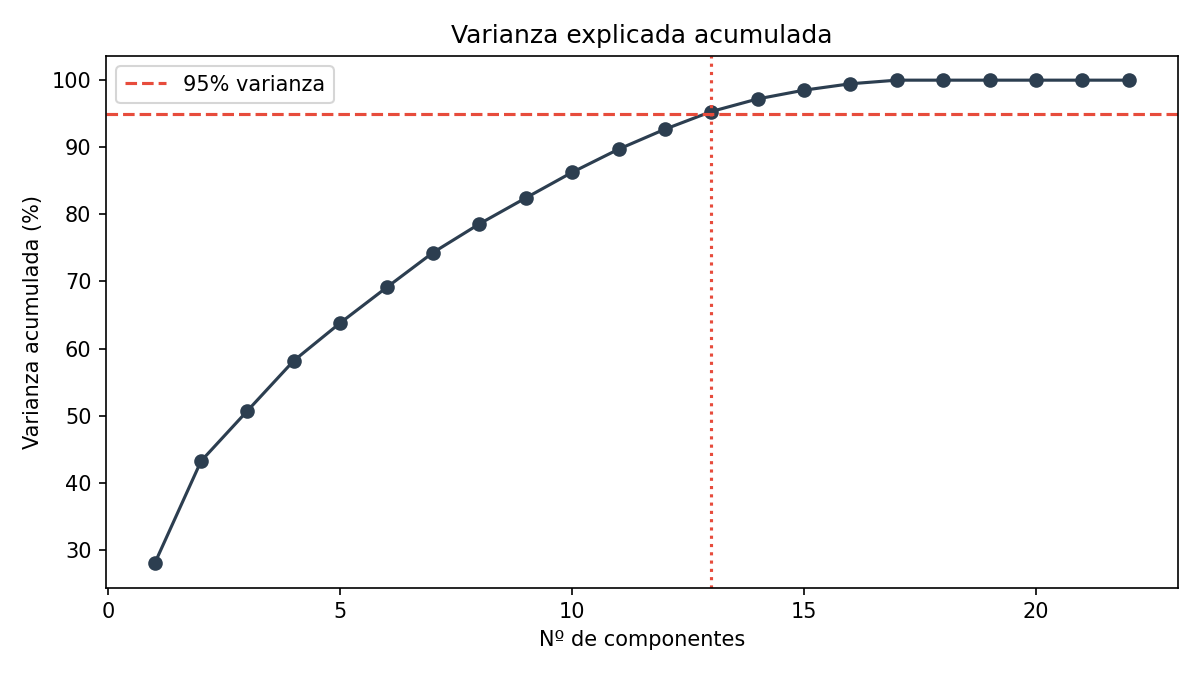
\includegraphics[width=0.86\linewidth]{pca_cumvar.png}
\caption{Varianza acumulada del an\'alisis de componentes principales sobre las variables
continuas. El 95\% se alcanza con 13 componentes; los cinco autovalores nulos reflejan la
colinealidad exacta de las variables de diferencia.}
\label{fig:pca}
\end{figure}

\section{Metodolog\'ia Propuesta}\label{sec:method}
La Fig.~\ref{fig:pipeline} resume el \emph{pipeline}. Sobre la matriz procesada se entrena
un conjunto de clasificadores, cuyos hiperpar\'ametros se seleccionan mediante validaci\'on
temporal interna, y el mejor de cada familia se compara sobre el conjunto de validaci\'on
antes de la evaluaci\'on final en prueba.

\begin{figure}[t]
\centering
\fbox{\parbox{0.92\linewidth}{\centering\footnotesize
Datos crudos $\rightarrow$ limpieza anti-fuga $\rightarrow$ reconstrucci\'on de Elo
$\rightarrow$ ingenier\'ia de \emph{features} $\rightarrow$ partici\'on temporal
$\rightarrow$ estandarizaci\'on (\emph{fit} en \emph{train}) $\rightarrow$
\{b\'usqueda de hiperpar\'ametros con \texttt{TimeSeriesSplit} $\rightarrow$ ajuste\}
$\rightarrow$ selecci\'on en validaci\'on $\rightarrow$ evaluaci\'on en prueba +
Wilcoxon + SHAP}}
\caption{Diagrama de bloques del \emph{pipeline} metodol\'ogico.}
\label{fig:pipeline}
\end{figure}

\subsection{Protocolo de validaci\'on y m\'etrica}
La selecci\'on de hiperpar\'ametros se realiza \emph{dentro} del entrenamiento con
\texttt{TimeSeriesSplit} de cinco pliegues expansivos, cuyo puntaje es el promedio de F1
macro:
\begin{equation}
\mathrm{CV}(\lambda)=\frac{1}{K}\sum_{i=1}^{K}\mathrm{F1}_{\text{macro}}\!\left(g^{-}_{\lambda,i}\right).
\end{equation}
La m\'etrica de optimizaci\'on es la \textbf{F1 macro}, que pondera por igual las tres
clases y penaliza ignorar el empate:
\begin{equation}
\mathrm{F1}_{\text{macro}}=\frac{1}{3}\sum_{c\in\{H,D,A\}}\frac{2P_cR_c}{P_c+R_c}.
\end{equation}
El reporte final incluye \emph{precision}, \emph{recall} y F1 por clase, el coeficiente
$\kappa$ de Cohen, el \'area bajo la curva ROC \emph{uno-contra-el-resto}, la matriz de
confusi\'on y la p\'erdida logar\'itmica.

\subsection{Modelos y fundamentos}
Se evaluaron nueve familias. Como \textbf{l\'ineas base}, un clasificador ingenuo
(clase mayoritaria) y \emph{Naive Bayes} gaussiano,
$\hat{y}=\arg\max_c P(c)\prod_j P(x_j\mid c)$, cuyo supuesto de independencia lo penaliza
en presencia de variables correlacionadas. Como \textbf{modelos lineales/de margen}, la
\textbf{regresi\'on log\'istica multinomial} con regularizaci\'on de Tikhonov,
\begin{equation}
\mathcal{L}=-\sum_i\log P(y_i\mid x_i)+\lambda\lVert W\rVert^2,
\end{equation}
donde el t\'ermino $\lambda\lVert W\rVert^2$ vuelve invertible la matriz singular por la
colinealidad; y la \textbf{m\'aquina de vectores de soporte}, que maximiza el margen
$1/\lVert w\rVert$ y cuyo \emph{kernel} de base radial
$K(x,x')=\exp(-\gamma\lVert x-x'\rVert^2)$ habilita fronteras no lineales.

Como \textbf{m\'etodos de \'arbol}, un \textbf{\'arbol de decisi\'on} que maximiza la
ganancia de informaci\'on $IG(Y,X)=H(Y)-H(Y\mid X)$; un \textbf{Random Forest}, cuya
varianza del promedio de $B$ \'arboles con correlaci\'on $\rho$ es
$\rho\sigma^2+\frac{1-\rho}{B}\sigma^2$, reducida al descorrelacionar mediante selecci\'on
aleatoria de atributos; y \textbf{AdaBoost}, que combina aprendices d\'ebiles con
$\alpha_m=\tfrac12\ln\frac{1-\epsilon_m}{\epsilon_m}$. Como \textbf{valor a\~nadido}, los
tres motores de \emph{gradient boosting} (XGBoost, LightGBM y CatBoost), que ajustan en
cada ronda un \'arbol al gradiente de la p\'erdida con regularizaci\'on de segundo orden:
\begin{equation}
\mathcal{L}^{(t)}\!\approx\!\sum_i\!\Big[g_i f_t(x_i)+\tfrac12 h_i f_t(x_i)^2\Big]+\gamma T+\tfrac12\lambda\lVert w\rVert^2,
\end{equation}
y un \textbf{ensamble} (\emph{voting} y \emph{stacking}) que, por el teorema del jurado de
Condorcet, mejora el consenso de modelos diversos.

\subsection{Selecci\'on de hiperpar\'ametros}
Cada hiperpar\'ametro clave se barre por curva de validaci\'on sobre
\texttt{TimeSeriesSplit}, eligiendo el punto donde la validaci\'on deja de mejorar (control
del compromiso sesgo--varianza). La Tabla~\ref{tab:hyper} resume los espacios de b\'usqueda;
los \emph{boosting} usan adem\'as parada temprana sobre el conjunto de validaci\'on. El
desbalance se maneja con \texttt{class\_weight} balanceado como estrategia primaria y con
SMOTE como experimento controlado. Todo el c\'omputo fija la semilla en 42.

\begin{table}[t]
\caption{Espacios de b\'usqueda de hiperpar\'ametros}
\label{tab:hyper}
\centering
\footnotesize
\begin{tabular}{@{}p{1.6cm}p{4.2cm}p{1.1cm}@{}}
\toprule
\textbf{Modelo} & \textbf{Rango} & \textbf{B\'usqueda} \\
\midrule
Log\'istica & $C\in\{10^{-2},\dots,10^{1}\}$, L2 & Grid \\
\'Arbol & \emph{max\_depth} 3--20, \emph{min\_leaf} 1--200 & Grid \\
SVM-RBF & $C\in\{0{,}1\dots100\}$, $\gamma\in\{$escala$,10^{-3}\dots1\}$ & Random \\
Random Forest & \emph{n\_est} 250--550, \emph{max\_feat} $\{$sqrt,0.3$\}$ & Random \\
XGB/LGBM & \emph{lr} 0.02--0.3, \emph{depth}, \emph{subsample} & Random \\
CatBoost & \emph{depth} 4--10, \emph{l2\_leaf\_reg} 1--10 & Random \\
\bottomrule
\end{tabular}
\end{table}

\section{Implementaci\'on del Software}\label{sec:software}
El sistema se implement\'o en Python~3.12 con \emph{scikit-learn}, XGBoost, LightGBM,
CatBoost, \emph{imbalanced-learn} y SHAP. El c\'odigo sigue una arquitectura modular en
\texttt{src/}, organizada por fase (\texttt{eda}, \texttt{preprocessing}, \texttt{modeling}),
donde cada modelo es un \emph{script} autocontenido que comparte un n\'ucleo com\'un
(\texttt{\_common.py}) con la carga de datos, el esquema de validaci\'on, el c\'alculo de
m\'etricas y la generaci\'on de figuras. La reproducibilidad determinista se garantiza
fijando la semilla global (\texttt{random\_state}=42) en Python, NumPy y en cada estimador,
b\'usqueda y pliegue. El entrenamiento de los modelos de \emph{boosting} se aceler\'o en
GPU (NVIDIA RTX 3060) mediante \texttt{device='cuda'} en XGBoost y \texttt{task\_type='GPU'}
en CatBoost. Cada \emph{script} vuelca sus m\'etricas y tiempos a \texttt{results/} y sus
figuras a \texttt{figures/}, y el cuaderno \texttt{3.0-modeling-evaluation.ipynb} reproduce
la metodolog\'ia de principio a fin sin errores.

En cuanto al costo computacional, la aceleraci\'on por GPU result\'o decisiva para los
modelos de \emph{boosting}: la b\'usqueda de hiperpar\'ametros de XGBoost sobre las 191\,099
instancias de entrenamiento requiri\'o del orden de siete minutos, y la de CatBoost, de
veinticuatro. LightGBM se ejecut\'o finalmente en CPU tras constatar que, en un conjunto de
este tama\~no, la recompilaci\'on del \emph{kernel} de c\'omputo en cada ajuste domina el
tiempo y anula la ventaja de la GPU. Los modelos lineales y de \'arbol se entrenaron en
segundos. El SVM de \emph{kernel} radial, cuyo costo es cuadr\'atico en el n\'umero de
muestras, se ajust\'o sobre una submuestra estratificada de 35\,000 partidos que preserva el
orden cronol\'ogico, decisi\'on documentada de forma expl\'icita para no ocultar el
submuestreo.

\section{Resultados Experimentales y An\'alisis Estad\'istico}\label{sec:results}
La Tabla~\ref{tab:results} presenta el desempe\~no en el conjunto de prueba (2024--2025),
ordenado por F1 macro. Todos los modelos competentes se agrupan en torno a un F1 macro de
0,42 y una exactitud de 0,44, coherente con el techo honesto de la literatura para la
predicci\'on previa al partido sin cuotas de mercado.

\begin{table}[t]
\caption{Resultados en el conjunto de prueba (2024--2025), ordenados por F1 macro}
\label{tab:results}
\centering
\footnotesize
\begin{tabular}{@{}lccccc@{}}
\toprule
\textbf{Modelo} & \textbf{F1$_\text{mac}$} & \textbf{Acc} & \textbf{$\kappa$} & \textbf{AUC} & \textbf{R$_D$} \\
\midrule
\textbf{Stacking (prop.)} & \textbf{0,419} & 0,438 & 0,146 & 0,610 & 0,264 \\
LightGBM        & 0,419 & 0,444 & 0,149 & 0,613 & 0,235 \\
Random Forest   & 0,417 & 0,446 & 0,149 & 0,614 & 0,213 \\
XGBoost         & 0,416 & 0,439 & 0,143 & 0,609 & 0,245 \\
CatBoost        & 0,415 & 0,442 & 0,146 & 0,615 & 0,221 \\
Voting          & 0,414 & 0,443 & 0,146 & 0,612 & 0,213 \\
SVM-RBF         & 0,413 & 0,424 & 0,134 & 0,606 & \textbf{0,314} \\
Reg. Log\'istica & 0,412 & 0,439 & 0,142 & 0,607 & 0,214 \\
\'Arbol         & 0,408 & 0,434 & 0,136 & 0,608 & 0,218 \\
AdaBoost        & 0,395 & 0,413 & 0,117 & 0,596 & 0,239 \\
Naive Bayes     & 0,392 & 0,412 & 0,103 & 0,576 & 0,235 \\
SVM lineal      & 0,335 & 0,472 & 0,113 & 0,604 & 0,004 \\
Dummy (piso)    & 0,202 & 0,434 & 0,000 & 0,500 & 0,000 \\
\bottomrule
\end{tabular}
\end{table}

La Tabla~\ref{tab:perclass} desglosa el F1 por clase para un subconjunto representativo de
modelos. El contraste es elocuente: la victoria local alcanza un F1 cercano a 0,52, mientras
que el empate no supera 0,31 en ning\'un caso. El SVM lineal ilustra el extremo pat\'ologico:
obtiene el mayor F1 de local (0,61) a costa de un F1 del empate pr\'acticamente nulo, es
decir, predice ``local'' de forma casi sistem\'atica. El SVM de \emph{kernel} radial, en
cambio, sacrifica algo de F1 en local para lograr el mejor desempe\~no en el empate.

\begin{table}[t]
\caption{F1 por clase en el conjunto de prueba (modelos seleccionados)}
\label{tab:perclass}
\centering
\footnotesize
\begin{tabular}{@{}lcccc@{}}
\toprule
\textbf{Modelo} & \textbf{F1$_H$} & \textbf{F1$_D$} & \textbf{F1$_A$} & \textbf{R$_D$} \\
\midrule
Stacking (prop.) & 0,515 & 0,280 & 0,462 & 0,264 \\
LightGBM        & 0,524 & 0,267 & 0,465 & 0,235 \\
SVM-RBF         & 0,482 & \textbf{0,305} & 0,453 & \textbf{0,314} \\
Reg. Log\'istica & 0,520 & 0,250 & 0,465 & 0,214 \\
SVM lineal      & \textbf{0,612} & 0,008 & 0,384 & 0,004 \\
\bottomrule
\end{tabular}
\end{table}

\subsection{La trampa de la exactitud}
La comparaci\'on con la l\'inea base ingenua es decisiva. El clasificador \emph{Dummy}, que
siempre predice la clase mayoritaria, alcanza una exactitud de 0,434 ---apenas por debajo
del 0,44 del mejor modelo---, pero su F1 macro es de solo 0,202 y su $\kappa$ es nulo. La
exactitud, por tanto, \emph{no} distingue un modelo \'util de uno in\'util en presencia de
desbalance. La superioridad real del sistema se manifiesta en el F1 macro (que se duplica),
en el coeficiente $\kappa$ (que pasa de 0 a $\approx0{,}15$) y en el AUC (de 0,50 a 0,61).
La Fig.~\ref{fig:compare} ilustra este contraste en validaci\'on y prueba.

\begin{figure}[t]
\centering
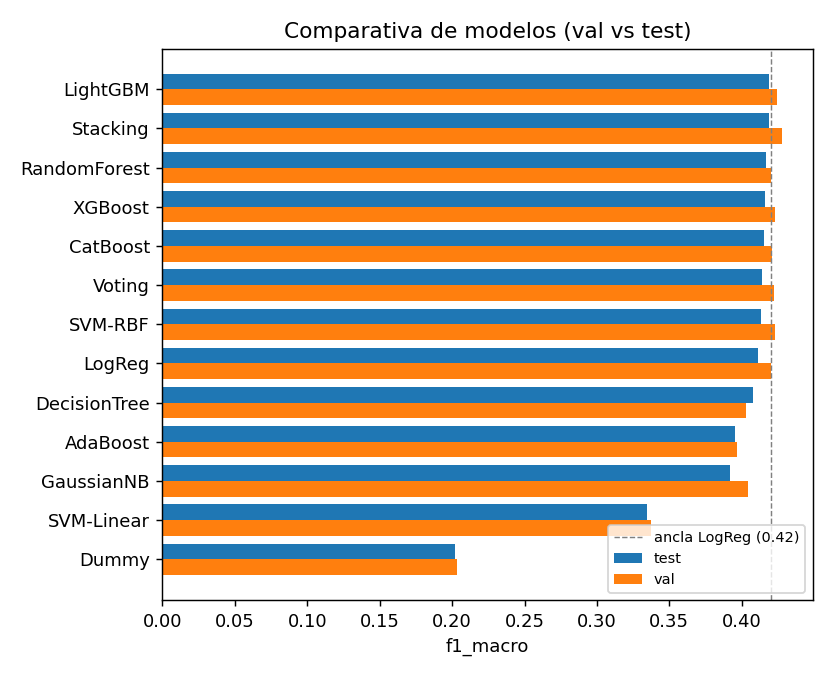
\includegraphics[width=0.94\linewidth]{11_model_comparison.png}
\caption{F1 macro por modelo en validaci\'on y prueba. La l\'inea de referencia marca el
ancla de la regresi\'on log\'istica; el pelot\'on ``real'' se agrupa muy por encima del
piso ingenuo (F1 macro 0,20).}
\label{fig:compare}
\end{figure}

\subsection{An\'alisis de la matriz de confusi\'on}
La matriz de confusi\'on del modelo propuesto (Fig.~\ref{fig:cm}) confirma la hip\'otesis
del an\'alisis exploratorio: el empate se confunde sistem\'aticamente con la victoria local
y la visitante, y casi nunca existe una regi\'on donde $D$ sea la predicci\'on
mayoritaria. Su sensibilidad m\'axima entre todos los modelos la alcanza el SVM de
\emph{kernel} radial (0,314), lo que refuerza la naturaleza no lineal de su frontera.

\begin{figure}[t]
\centering
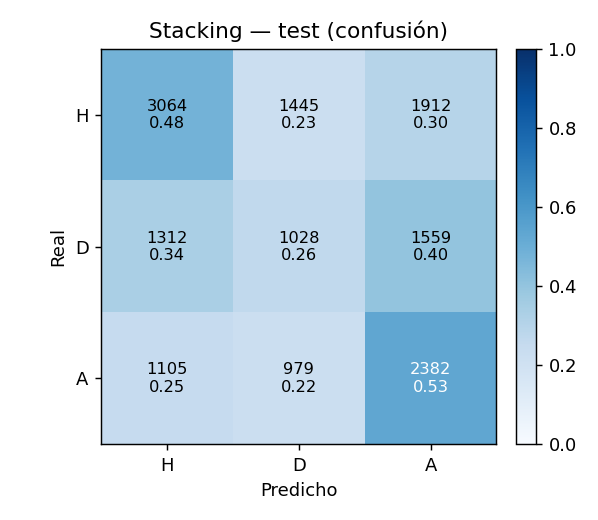
\includegraphics[width=0.68\linewidth]{cm_11_proposed_test.png}
\caption{Matriz de confusi\'on del modelo propuesto (Stacking) en prueba. El empate se
reparte entre local y visitante, evidenciando su techo estructural.}
\label{fig:cm}
\end{figure}

\subsection{Experimento de desbalance}
La Tabla~\ref{tab:imbalance} compara tres estrategias con una configuraci\'on de XGBoost
fija. Sin balanceo, el modelo pr\'acticamente no predice empates (sensibilidad de $D$ de
0,008), a pesar de una exactitud mayor. El reponderado por clase es la \'unica estrategia
que eleva simult\'aneamente el F1 macro y la sensibilidad del empate. SMOTE apenas ayuda:
al interpolar entre empates ---adem\'as sobre variables \emph{one-hot}--- genera puntos que
caen en zonas ya dominadas por otras clases, sin crear frontera nueva, coherente con la
ausencia de regi\'on propia del empate.

\begin{table}[t]
\caption{Estrategias de desbalance (XGBoost fijo, validaci\'on)}
\label{tab:imbalance}
\centering
\footnotesize
\begin{tabular}{@{}lccc@{}}
\toprule
\textbf{Estrategia} & \textbf{F1 macro} & \textbf{Recall $D$} & \textbf{Exactitud} \\
\midrule
Sin balanceo   & 0,348 & 0,008 & 0,484 \\
\texttt{class\_weight} & \textbf{0,425} & \textbf{0,243} & 0,449 \\
SMOTE          & 0,356 & 0,016 & 0,484 \\
\bottomrule
\end{tabular}
\end{table}

\subsection{Interpretabilidad}
El an\'alisis SHAP sobre el modelo de \emph{boosting} (Fig.~\ref{fig:shap}) identifica la
\textbf{diferencia de Elo} como la variable dominante, muy por encima del historial directo,
la forma reciente y el balance de goles. Este resultado coincide con la importancia por
permutaci\'on del \emph{Random Forest} y confirma cuantitativamente la lectura del an\'alisis
exploratorio: la diferencia de calidad entre equipos explica la mayor parte de lo predecible.

\begin{figure}[t]
\centering
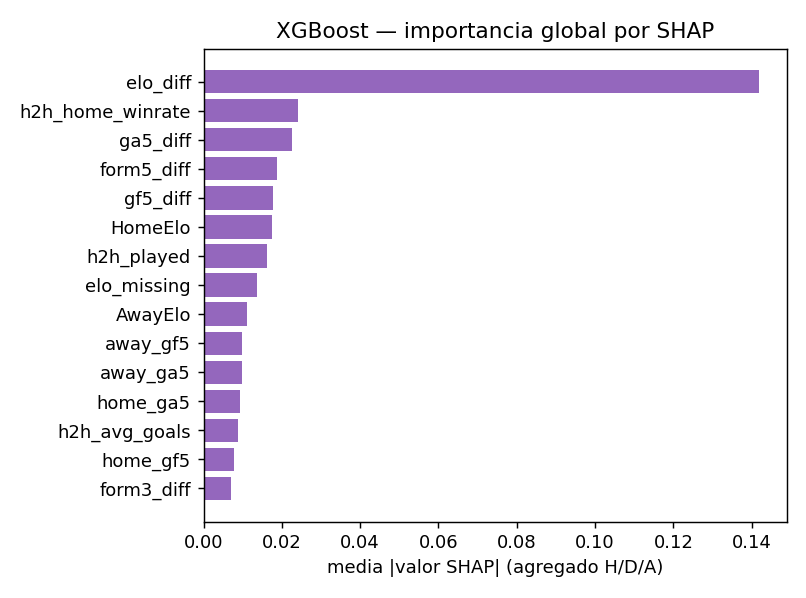
\includegraphics[width=0.92\linewidth]{shap_importance.png}
\caption{Importancia global por valores SHAP sobre XGBoost. La diferencia de Elo domina la
predicci\'on, seguida del historial directo y la forma reciente.}
\label{fig:shap}
\end{figure}

Este hallazgo se corrobora con un m\'etodo independiente: la importancia por permutaci\'on
del \emph{Random Forest} (Fig.~\ref{fig:permimp}), que mide la ca\'ida de F1 macro al
permutar cada variable, sit\'ua nuevamente a la diferencia de Elo muy por delante del resto.
La coincidencia de dos t\'ecnicas de atribuci\'on distintas refuerza la robustez de la
conclusi\'on.

\begin{figure}[t]
\centering
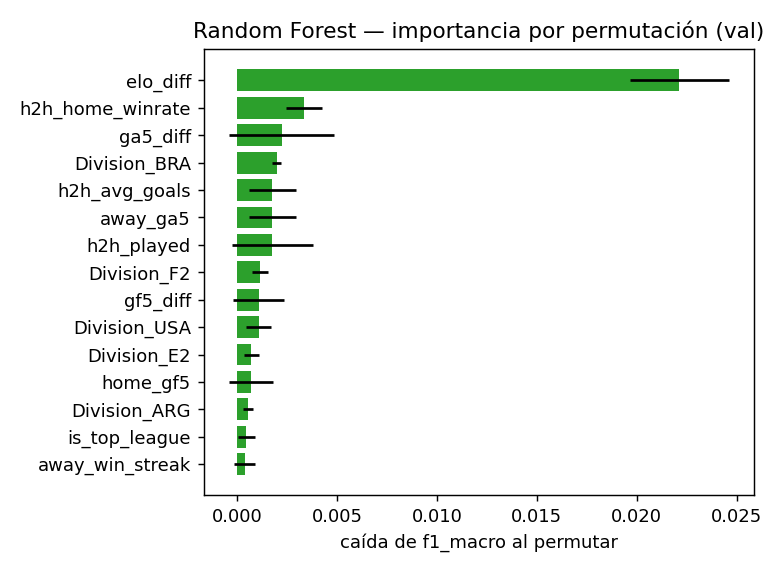
\includegraphics[width=0.94\linewidth]{permimp_03_rf.png}
\caption{Importancia por permutaci\'on del \emph{Random Forest} sobre validaci\'on. La
ca\'ida de F1 macro al permutar la diferencia de Elo supera con creces a la del resto de
variables, en coincidencia con el an\'alisis SHAP.}
\label{fig:permimp}
\end{figure}

\subsection{Significancia estad\'istica}
Para descartar que la ventaja del modelo propuesto sea producto del azar, se aplic\'o la
prueba de Wilcoxon de rangos con signo ($\alpha=0{,}05$) sobre el F1 macro calculado por
bloque temporal mensual en el conjunto de prueba ($n=17$ bloques). El \emph{stacking}
supera al clasificador ingenuo ($p=7{,}6\times10^{-6}$) y al \emph{Naive Bayes}
($p=6{,}7\times10^{-4}$), ambos resultados estad\'isticamente significativos. La mejora,
por tanto, es consistente a lo largo del tiempo y no atribuible a variabilidad experimental.

\section{Discusi\'on}\label{sec:discussion}
Los resultados admiten una lectura unificada a partir de las propiedades detectadas en el
an\'alisis exploratorio. El liderazgo (marginal) de los m\'etodos de \emph{boosting} y del
ensamble, junto con el contraste entre el SVM lineal ---que hunde la sensibilidad del empate
a casi cero--- y el SVM de \emph{kernel} radial ---que la eleva a 0,31---, confirma que la
frontera de decisi\'on es no lineal. Sin embargo, la agrupaci\'on estrecha de todos los
modelos competentes indica que, en ausencia de cuotas de mercado, la se\~nal disponible tiene
un techo bajo, y ning\'un algoritmo lo supera de forma dram\'atica. El empate act\'ua como
muro estructural: no ocupa una regi\'on propia del espacio de \emph{features}, por lo que su
sensibilidad est\'a acotada con independencia del clasificador. El \emph{stacking} obtiene la
mejor F1 macro porque su meta-modelo aprende a ponderar la fortaleza de cada base seg\'un la
regi\'on del espacio.

\textbf{Amenazas a la validez interna.} El principal riesgo, la fuga temporal, se mitiga con
la partici\'on por fecha y la validaci\'on con \texttt{TimeSeriesSplit}; la ausencia de
exactitudes sospechosamente altas ($>65\%$) es coherente con un pipeline sin fuga. El
ensamble por apilamiento emplea un esquema de validaci\'on interno estratificado para generar
las predicciones fuera de pliegue, mientras la integridad temporal se preserva en el nivel
externo, con validaci\'on y prueba intactas.

\textbf{Amenazas a la validez externa.} El modelo se entren\'o sin cuotas de mercado, por lo
que su techo es inherentemente inferior al de sistemas que las incorporan; su capacidad de
generalizaci\'on a ligas o temporadas con din\'amicas muy distintas (por ejemplo, la deriva
observada durante la pandemia) no est\'a garantizada. Adem\'as, la ausencia estructural de
Elo en ligas no europeas limita la homogeneidad de la se\~nal entre competiciones.

\subsection{Consideraciones \'eticas}
El conjunto de datos no contiene atributos personales sensibles ---g\'enero, etnia o
condici\'on socioecon\'omica de individuos---: las entidades son clubes y sus estad\'isticas
deportivas agregadas, por lo que no procede un an\'alisis de sesgos demogr\'aficos. No
obstante, un sistema de predicci\'on de resultados deportivos puede emplearse en mercados de
apuestas; su uso responsable exige comunicar con transparencia la elevada incertidumbre del
modelo ---evidenciada por el techo de rendimiento--- y no presentarlo como una herramienta
de ganancia garantizada.

\section{Conclusiones y Trabajo Futuro}\label{sec:conclusions}
Este trabajo present\'o una comparaci\'on emp\'irica reproducible de nueve familias de
clasificadores para la predicci\'on multiclase de resultados de f\'utbol sobre 230\,554
partidos multi-liga, con un protocolo de validaci\'on temporal y m\'etricas robustas al
desbalance. Las conclusiones t\'ecnicas son tres. Primero, el empate constituye un l\'imite
estructural: ning\'un modelo super\'o un F1 macro global de 0,42 ni una sensibilidad del
empate por encima de 0,33, no por deficiencia de los algoritmos sino por la geometr\'ia del
problema. Segundo, la frontera es no lineal, como evidencian el contraste SVM lineal frente
a \emph{kernel} radial y el liderazgo del \emph{boosting} y el \emph{stacking}; el
reponderado por clase result\'o superior al sobremuestreo sint\'etico, y la diferencia de
Elo es la variable dominante seg\'un SHAP. Tercero, el modelo propuesto supera a las l\'ineas
base con significancia estad\'istica, lo que valida la contribuci\'on frente al azar
experimental.

Como trabajo futuro se plantea incorporar las cuotas de mercado como \emph{features} para
cuantificar el salto de rendimiento respecto de la versi\'on honesta, modelar la
incertidumbre del empate mediante salidas probabil\'isticas calibradas y la m\'etrica RPS,
y explorar arquitecturas secuenciales que capturen la forma de los equipos como serie
temporal.

\begin{thebibliography}{00}
\bibitem{rodrigues2022} F. Rodrigues and \^A. Pinto, ``Prediction of football match results with Machine Learning,'' \emph{Procedia Computer Science}, vol. 204, pp. 463--470, 2022.
\bibitem{bunker2019} R. Bunker and F. Thabtah, ``A machine learning framework for sport result prediction,'' \emph{Applied Computing and Informatics}, vol. 15, no. 1, pp. 27--33, 2019.
\bibitem{ren2022} Y. Ren and T. Susnjak, ``Predicting football match outcomes with explainable machine learning,'' \emph{arXiv:2211.15734}, 2022.
\bibitem{bunker2024} R. Bunker, C. Yeung, and K. Fujii, ``Machine learning in sports: A survey and future directions,'' \emph{arXiv:2403.07669}, 2024.
\bibitem{choi2023} B. Choi, L. Foo, and G. Chua, ``Predicting football match outcomes with machine learning approaches,'' \emph{MENDEL}, vol. 29, no. 2, pp. 229--236, 2023.
\bibitem{stubinger2020} J. St\"ubinger, B. Mangold, and J. Knoll, ``Machine learning in football betting: Prediction of match results based on player characteristics,'' \emph{Applied Sciences}, vol. 10, no. 1, art. 46, 2020.
\bibitem{yeung2023} C. Yeung, R. Bunker, and K. Fujii, ``A framework of interpretable match results prediction in football,'' \emph{PLOS ONE}, vol. 18, no. 4, e0284318, 2023.
\bibitem{berrar2019} D. Berrar, P. Lopes, and W. Dubitzky, ``Incorporating domain knowledge in machine learning for soccer outcome prediction,'' \emph{Machine Learning}, vol. 108, pp. 97--126, 2019.
\bibitem{berrar2024} D. Berrar, P. Lopes, and W. Dubitzky, ``Predicting soccer results through ensemble learning,'' \emph{Machine Learning}, vol. 113, 2024.
\bibitem{attamills2024} E. F. E. Atta Mills \emph{et al.}, ``Football match outcome prediction using machine learning,'' \emph{Journal of Big Data}, vol. 11, art. 170, 2024.
\bibitem{constantinou2013} A. C. Constantinou and N. E. Fenton, ``Determining the level of ability of football teams by dynamic ratings,'' \emph{Journal of Quantitative Analysis in Sports}, vol. 9, no. 1, pp. 37--50, 2013.
\bibitem{dixon1997} M. J. Dixon and S. G. Coles, ``Modelling association football scores and inefficiencies in the football betting market,'' \emph{Applied Statistics}, vol. 46, no. 2, pp. 265--280, 1997.
\bibitem{hvattum2010} L. M. Hvattum and H. Arntzen, ``Using ELO ratings for match result prediction in association football,'' \emph{International Journal of Forecasting}, vol. 26, no. 3, pp. 460--470, 2010.
\bibitem{chawla2002} N. V. Chawla, K. W. Bowyer, L. O. Hall, and W. P. Kegelmeyer, ``SMOTE: Synthetic Minority Over-sampling Technique,'' \emph{Journal of Artificial Intelligence Research}, vol. 16, pp. 321--357, 2002.
\bibitem{lundberg2017} S. M. Lundberg and S.-I. Lee, ``A unified approach to interpreting model predictions,'' in \emph{Advances in Neural Information Processing Systems}, vol. 30, 2017.
\bibitem{chen2016} T. Chen and C. Guestrin, ``XGBoost: A scalable tree boosting system,'' in \emph{Proc. 22nd ACM SIGKDD}, 2016, pp. 785--794.
\bibitem{ke2017} G. Ke \emph{et al.}, ``LightGBM: A highly efficient gradient boosting decision tree,'' in \emph{Advances in Neural Information Processing Systems}, vol. 30, 2017.
\bibitem{prokhorenkova2018} L. Prokhorenkova \emph{et al.}, ``CatBoost: unbiased boosting with categorical features,'' in \emph{Advances in Neural Information Processing Systems}, vol. 31, 2018.
\bibitem{breiman2001} L. Breiman, ``Random forests,'' \emph{Machine Learning}, vol. 45, no. 1, pp. 5--32, 2001.
\bibitem{pedregosa2011} F. Pedregosa \emph{et al.}, ``Scikit-learn: Machine learning in Python,'' \emph{Journal of Machine Learning Research}, vol. 12, pp. 2825--2830, 2011.
\end{thebibliography}

\end{document}
